\documentclass[11pt]{article}
\usepackage{amsmath,textcomp,amssymb,graphicx,comment,tikz}
\usepackage[margin=0.75in]{geometry}
\usetikzlibrary{arrows}
\newcommand{\tab}{\hspace*{2em}}

\def\Name{Alvin Wong (22655478, -cq) , Wai Meng Lei (23985541, -dy) , Chun Yin Yau (24023460, -em)}  % Your name

\title{CS189 --- Homework 7}
\author{\Name}
\markboth{CS189 Homework 7}{CS189 Homework 7}
\pagestyle{myheadings}

\begin{document}
\maketitle
\vspace{5em}
\section*{1. K-Means Clustering on MNIST (page 1 out of 4)}
The code can be run in the code directory, by running the command hw7q1. Note that this may take a while since we use the full 60k MNIST dataset. We initialized the cluster centers to be randomly chosen from the datapoints provided in the training set -- this helps us with preventing clusters with no points. The images for the means are posted below:
\\\\
a) $k = 5$:
\begin{figure}[ht!]
\centering
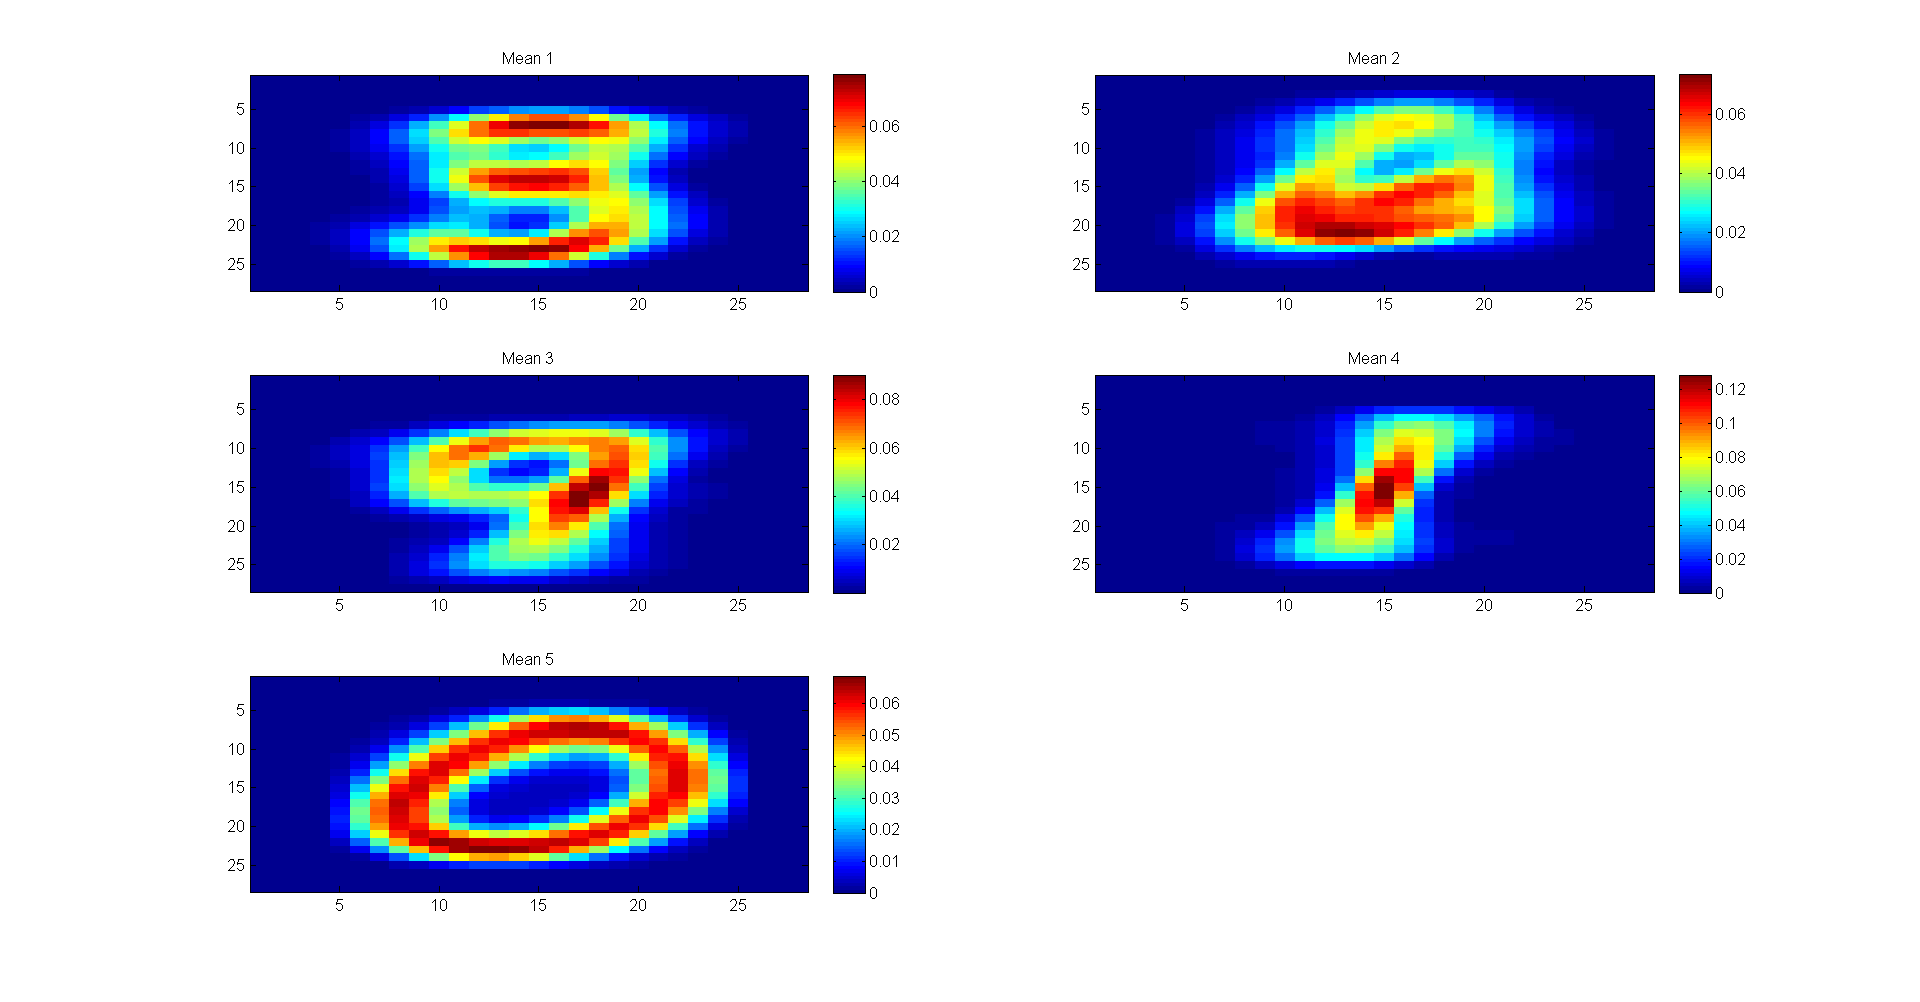
\includegraphics[width=180mm]{images/mean5-1.png}
\label{overflow}
\end{figure}
\newpage
\section*{1. K-Means Clustering on MNIST (page 2 out of 4)}
b) $k=10$:
\begin{figure}[ht!]
\centering
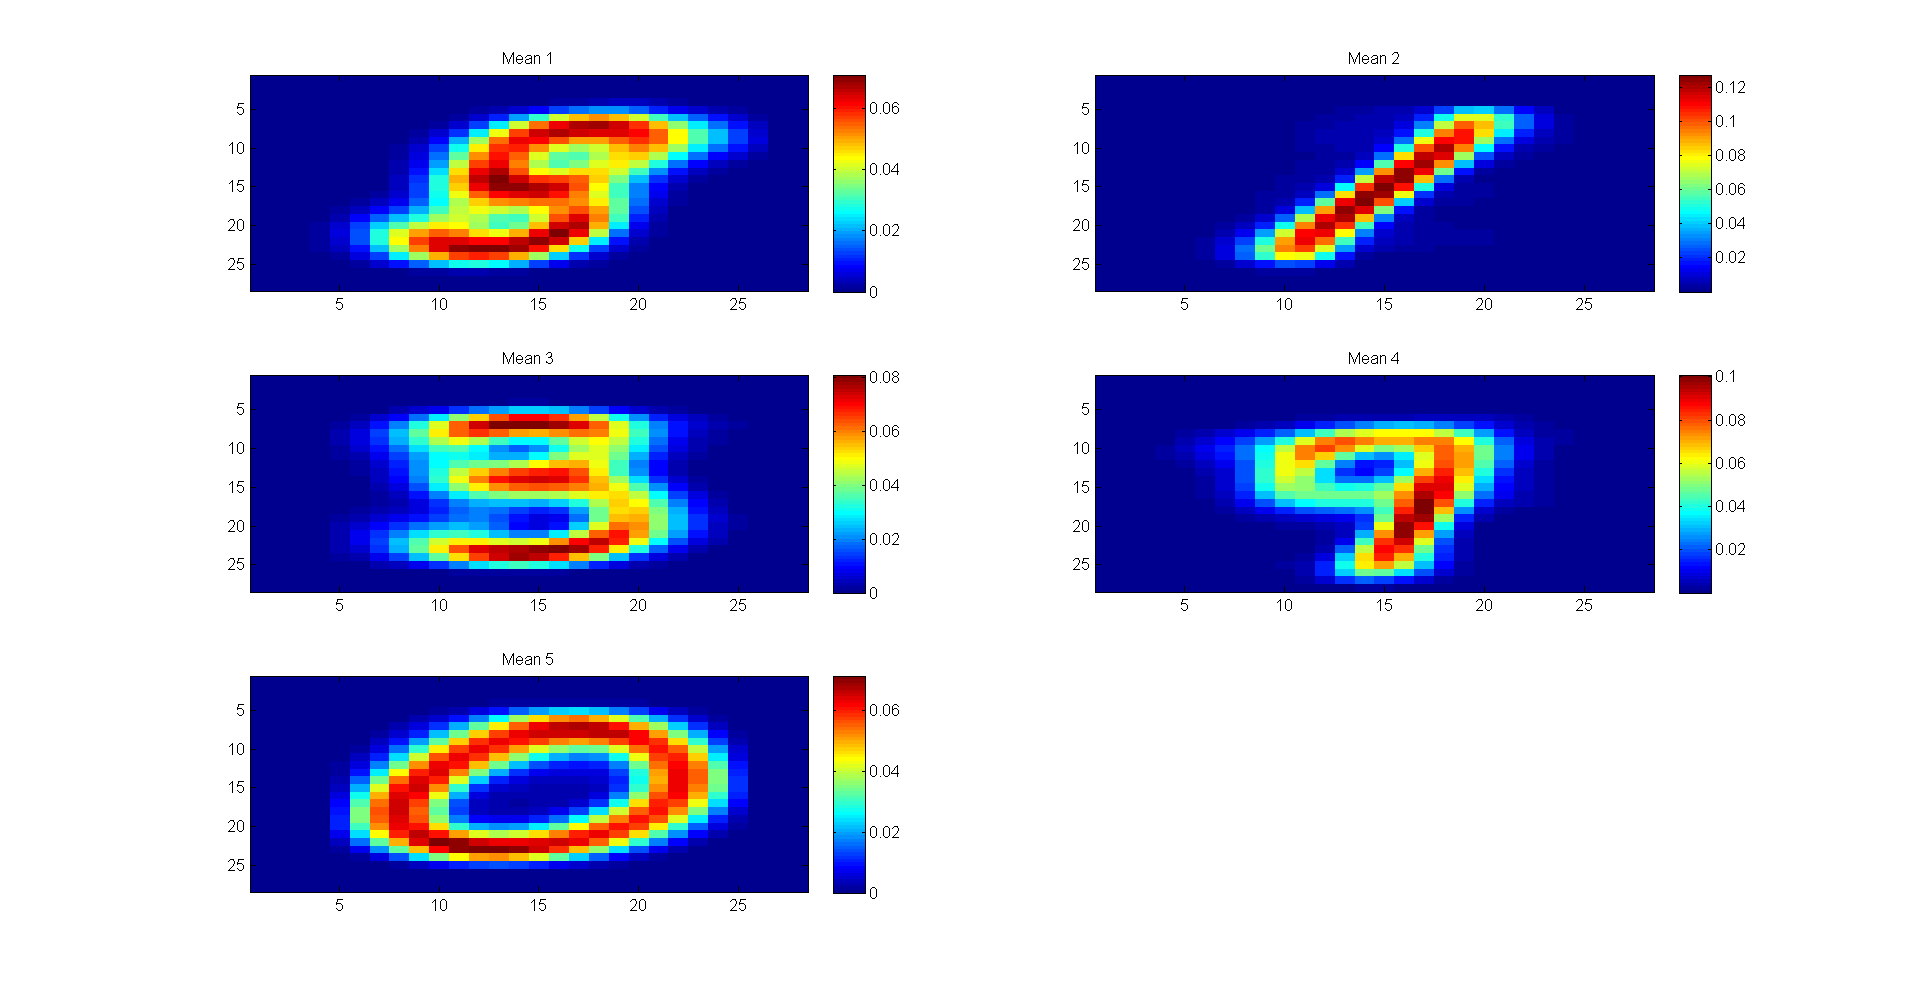
\includegraphics[width=180mm]{images/mean10-1.png}
\label{overflow}
\end{figure}
\begin{figure}[ht!]
\centering
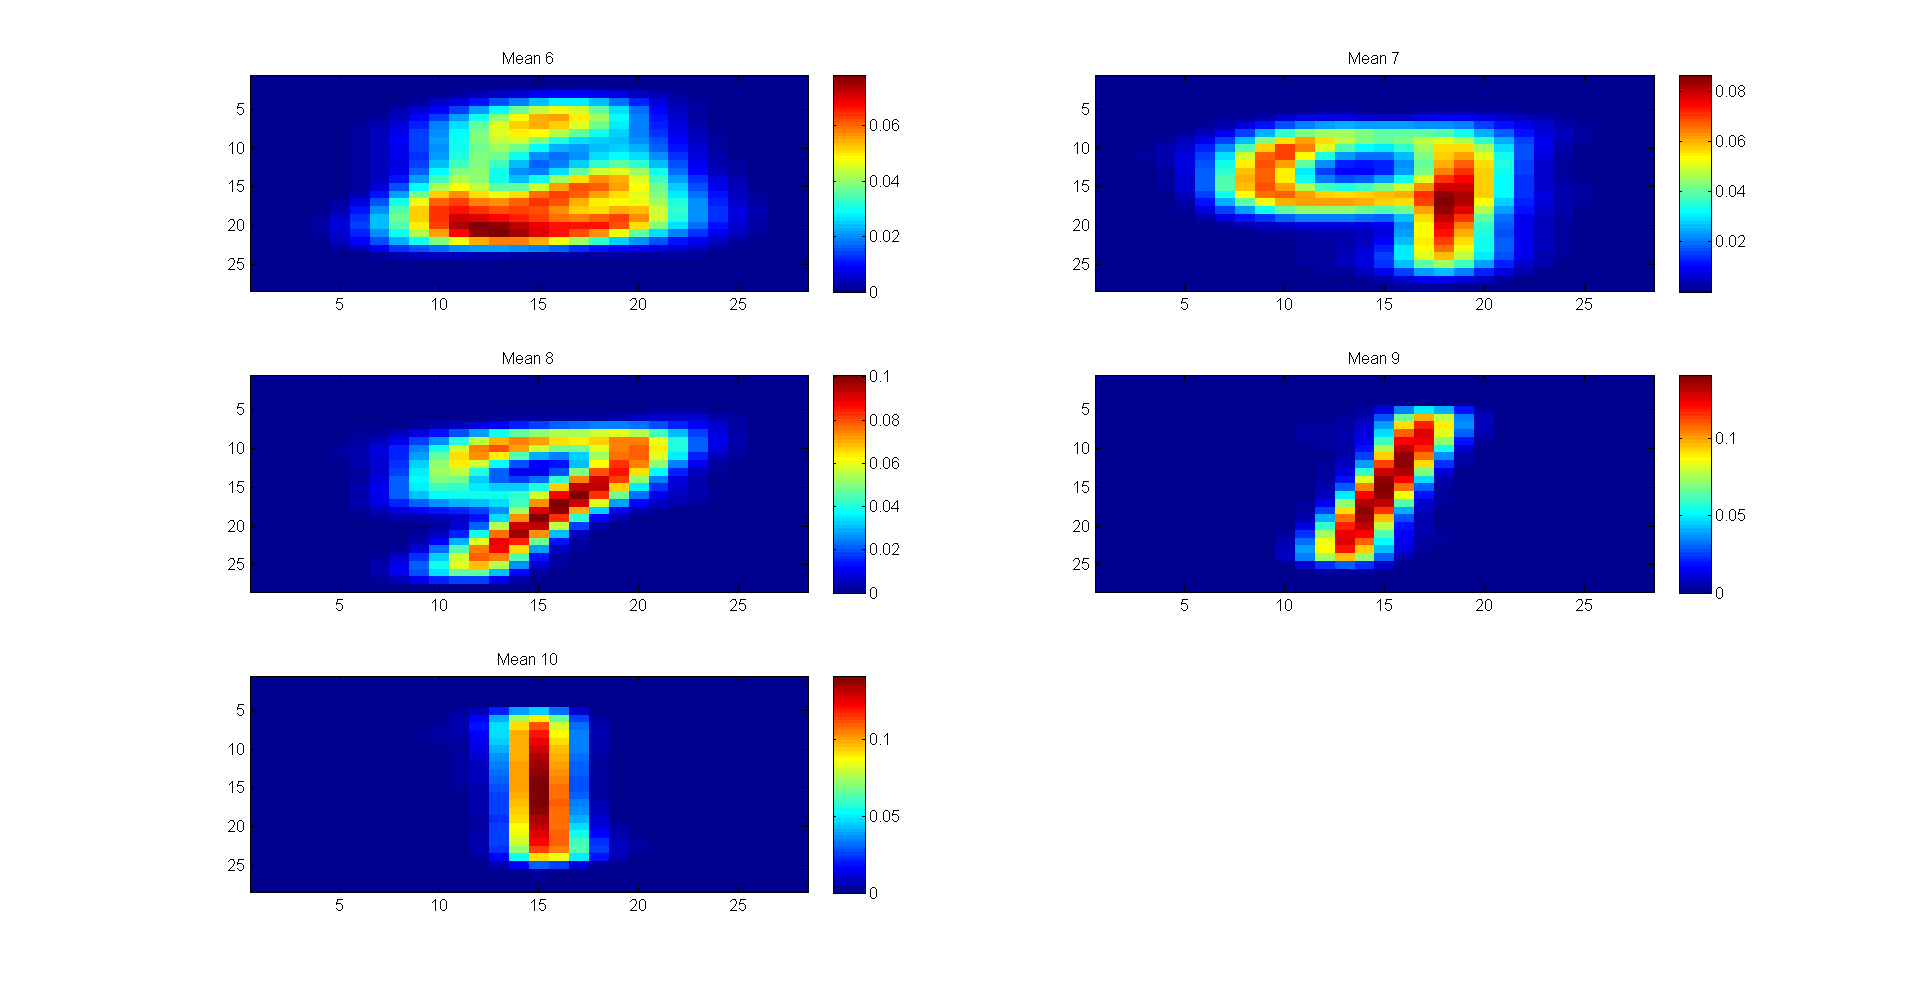
\includegraphics[width=180mm]{images/mean10-2.png}
\label{overflow}
\end{figure}
\newpage
\section*{1. K-Means Clustering on MNIST (page 3 out of 4)}
c) $k=20$:
\begin{figure}[ht!]
\centering
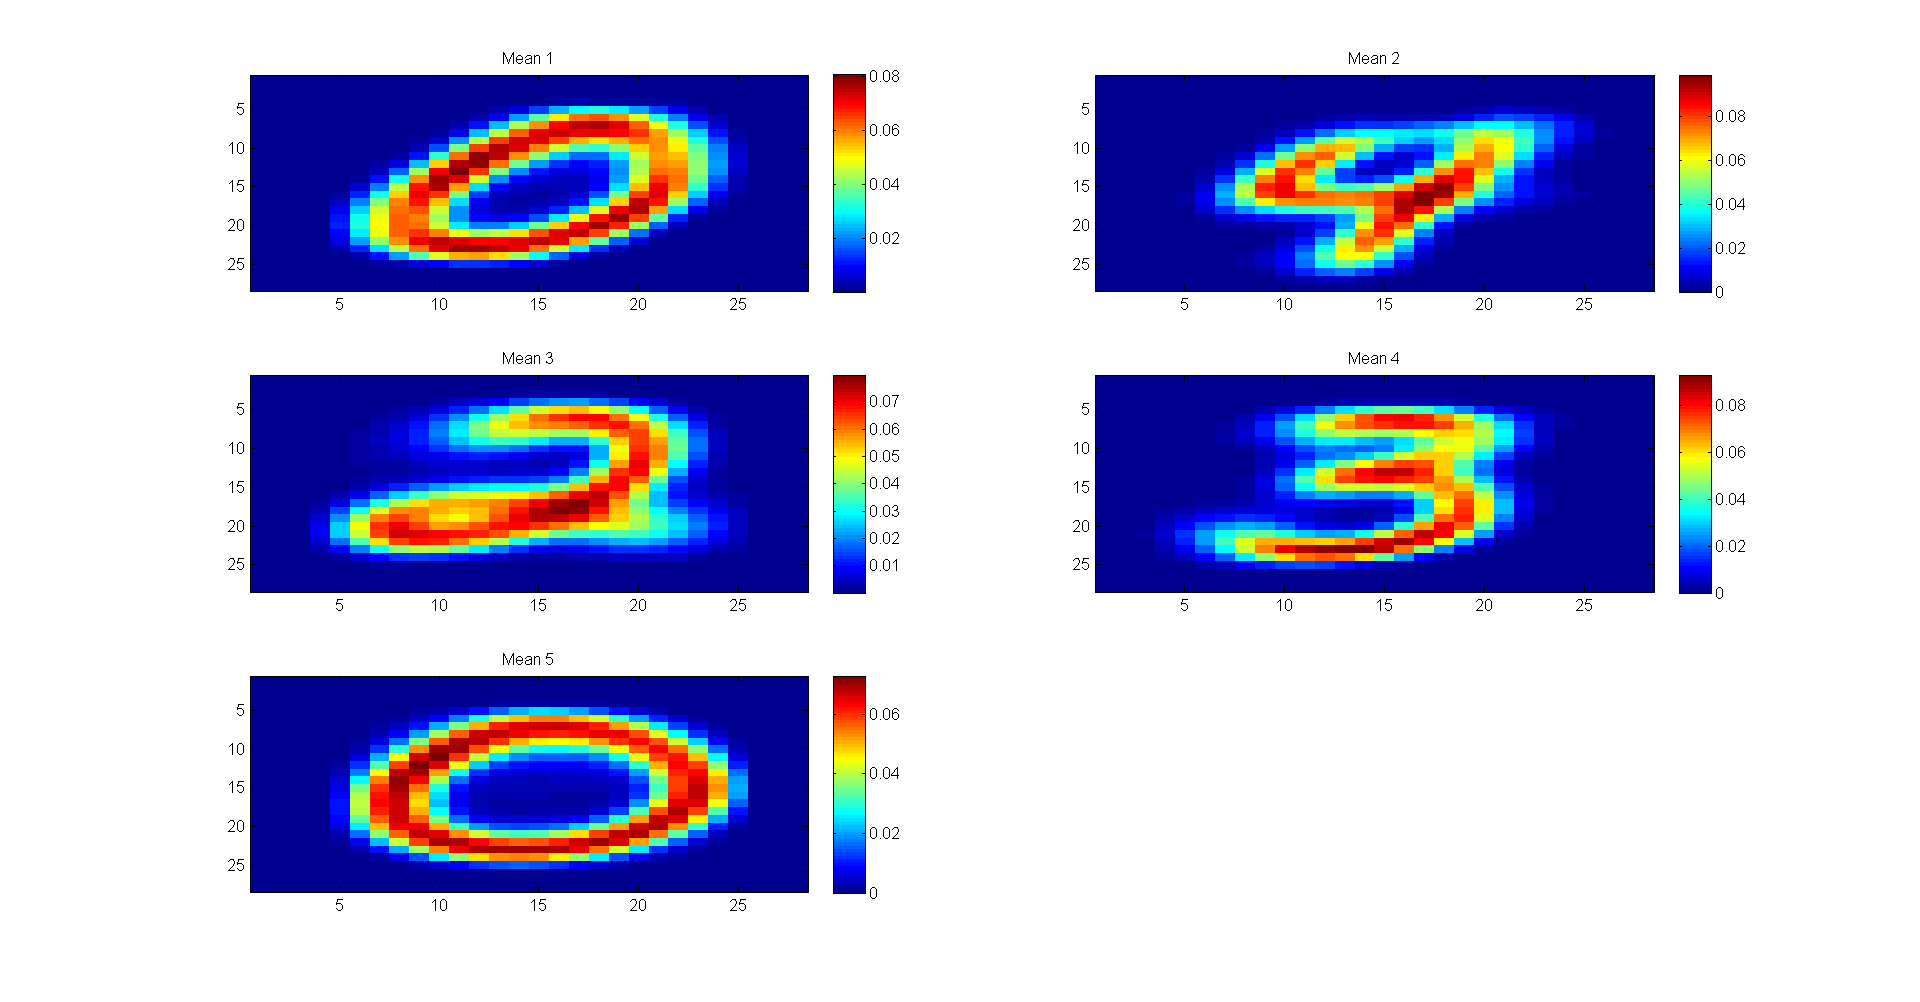
\includegraphics[width=180mm]{images/mean20-1.png}
\label{overflow}
\end{figure}
\begin{figure}[ht!]
\centering
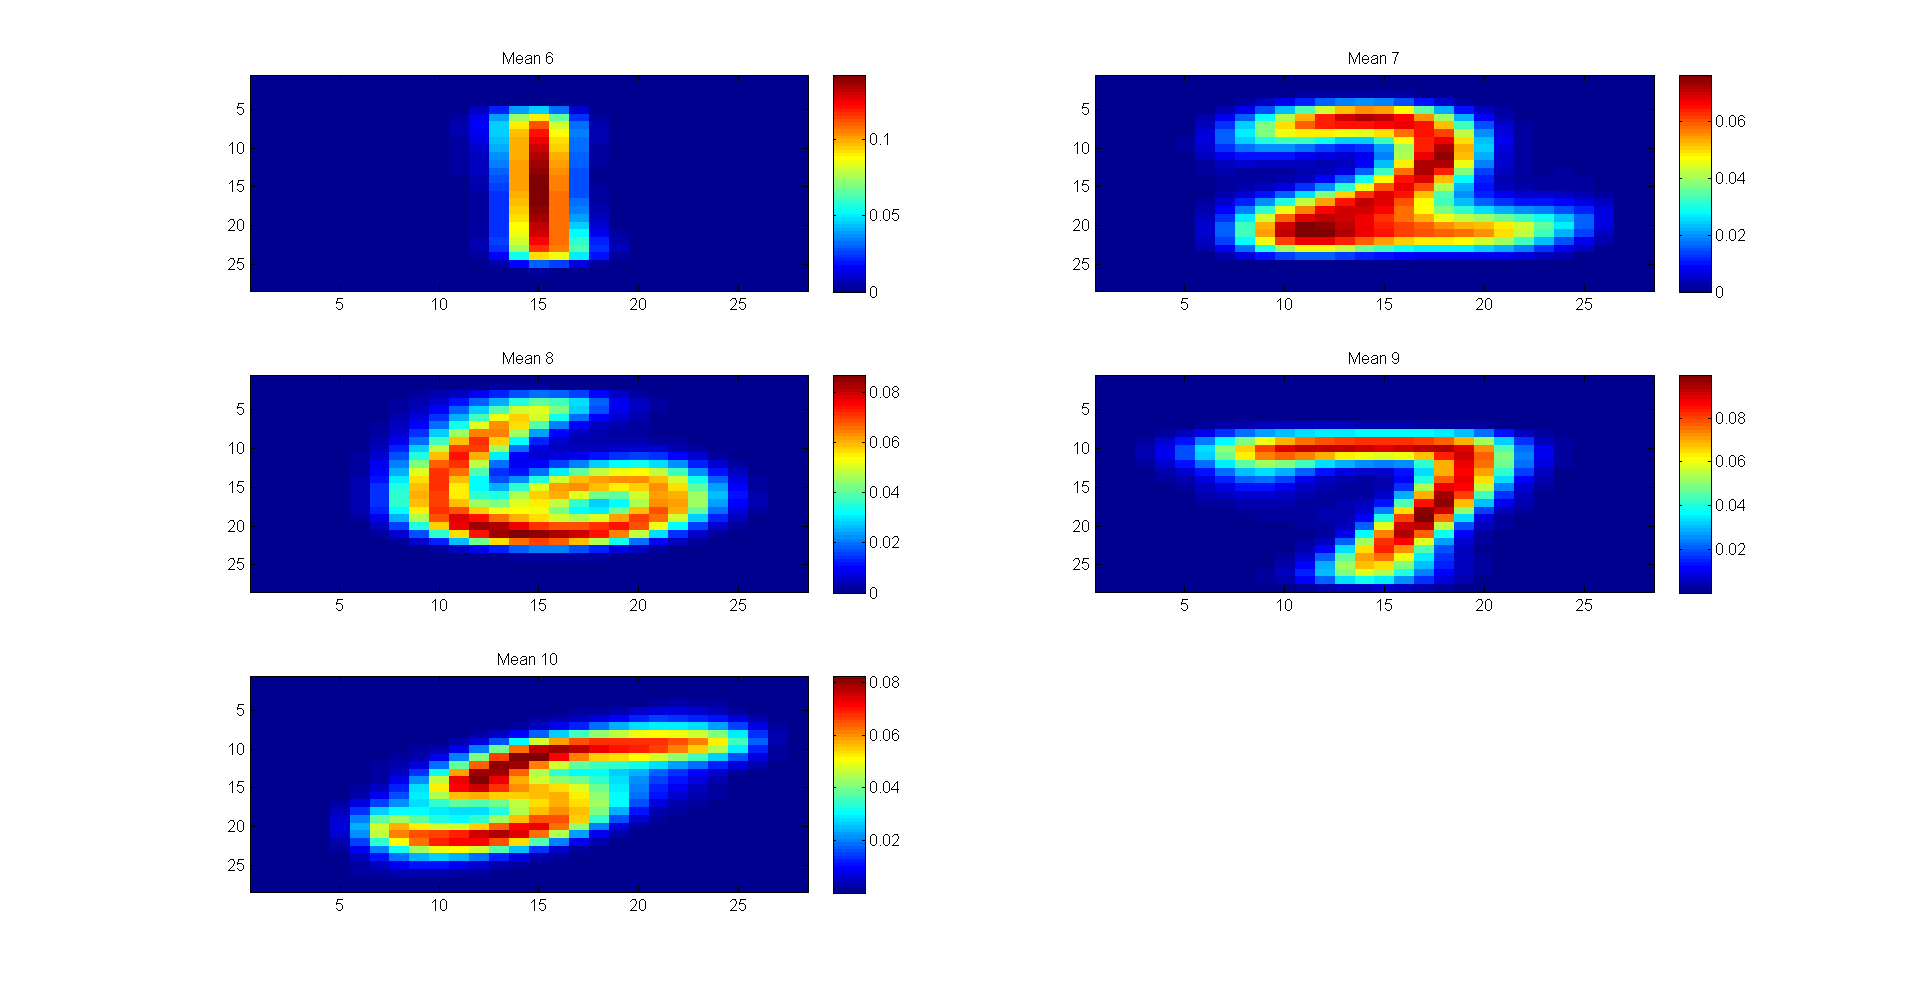
\includegraphics[width=180mm]{images/mean20-2.png}
\label{overflow}
\end{figure}
\newpage
\section*{1. K-Means Clustering on MNIST (page 4 out of 4)}
c) $k=20$ (continued):
\begin{figure}[ht!]
\centering
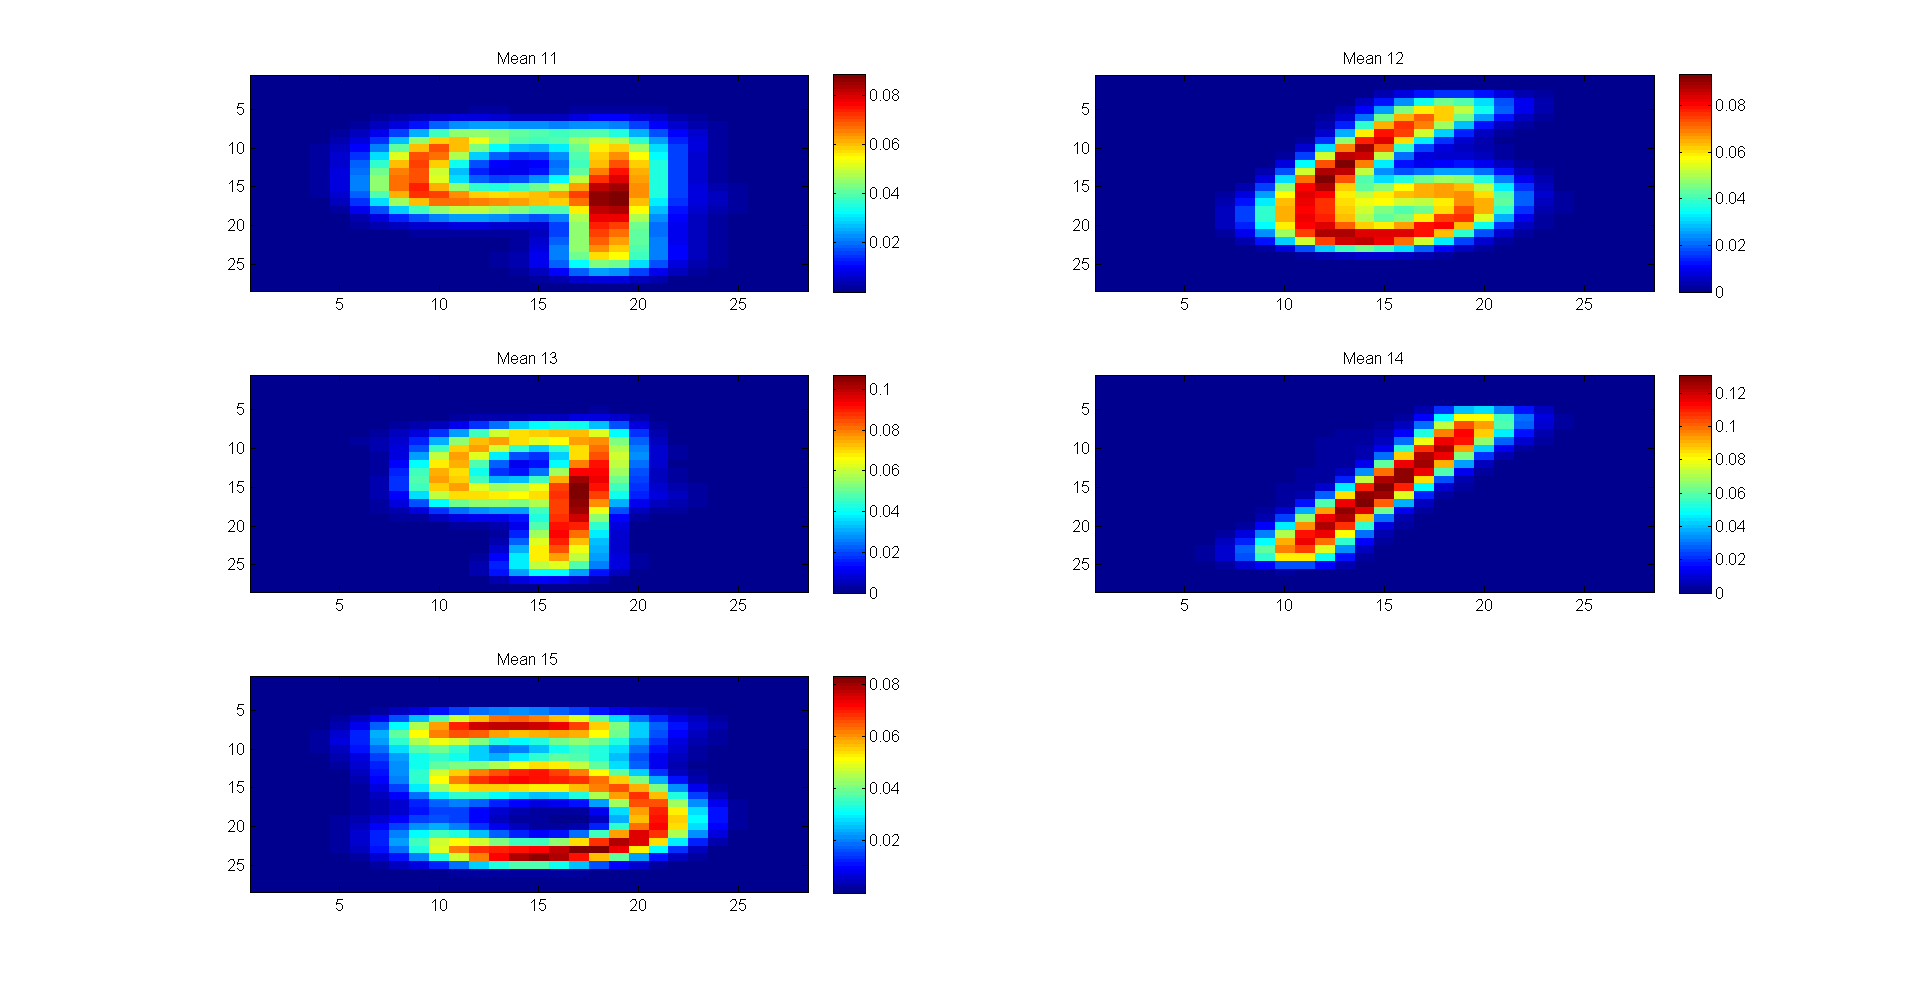
\includegraphics[width=180mm]{images/mean20-3.png}
\label{overflow}
\end{figure}
\begin{figure}[ht!]
\centering
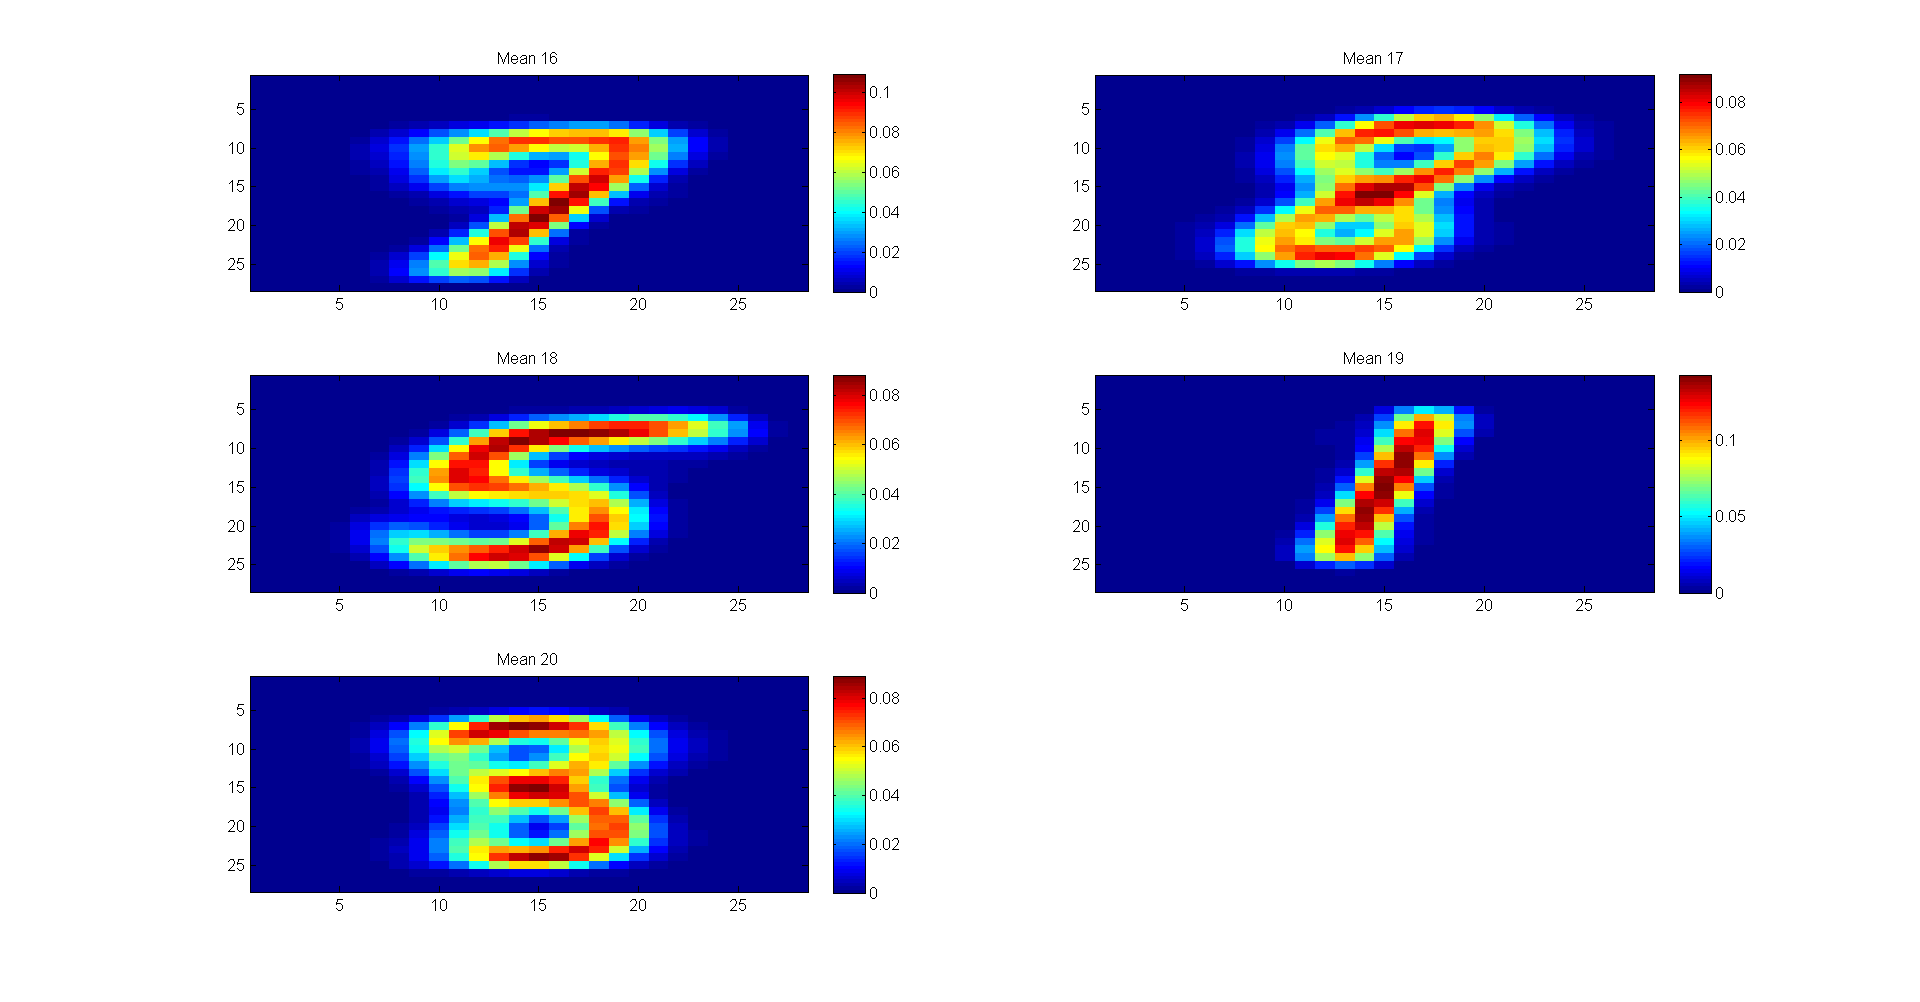
\includegraphics[width=180mm]{images/mean20-4.png}
\label{overflow}
\end{figure}
\newpage

\section*{2. Eigenfaces (page 1 out of 7)}
(a) The top 10 eigenfaces are as follows, ranked from 1 to 10:
\\\\
Top 1-5:
\begin{figure}[ht!]
\centering
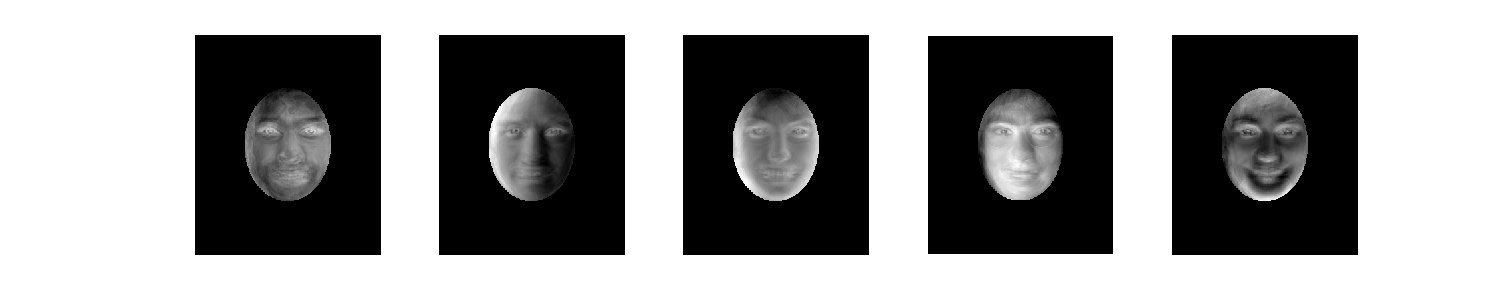
\includegraphics[width=180mm]{images/eigface5-1.png}
\label{overflow}
\end{figure}
\\
(1) This eigenface shows the facial features -- the eyes are light, the hair and facial hair are darker. Doesn't include much llight shading. \\
(2) This eigenface captures the lighting on the right side of the face (left side of the image), and the shadow on the left side of the face (right side of the image). \\
(3) This eigenface captures the lighting of the lower left and right sides of the face and the dark part of the hair. Also has some facial expressions at the mouth. \\
(4) This eigenface captures the illumination in the front of the face. It shows the nose bulging outwards as well. \\
(5) This eigenface captures the shadow below the mouth, eyes, and on the nose.
\\\\
Top 6-10:
\begin{figure}[ht!]
\centering
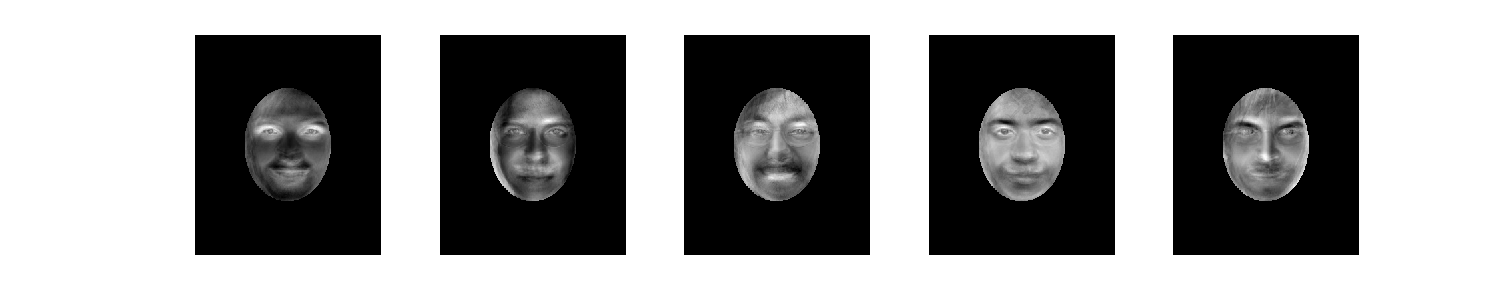
\includegraphics[width=180mm]{images/eigface5-2.png}
\label{overflow}
\end{figure}
\\
(6) This eigenface captures the lighting in the eyes, the shadows under the nose, and the dark parts of facial hair. \\
(7) This eigenface captures the illumination on the right side of the face, a bit of lighting in the front of the face (near the nose and forehead), and outline of the mouth. Also can see outline of glasses. \\
(8) This eigenface has a moustache. It also has a band of illumination accross the front of the head, dark part for hair, and outline of glasses. \\
(9) This eigenface captures a mouth shape and the shadows near the mouth. It also captures the illumination across the front face. \\
(10) This eigenface has a lot of light contrast on the nose area, and heavy contrast across the eyes and eyebrows. Also a bit of illumination on the left side of the face.
\\\\
Run hw7q2a in the code subdirectory if you want to see the implementation. (Shouldn't take more than 5 seconds).
\newpage

\section*{2. Eigenfaces (page 2 out of 7)}
(b) To reconstruct the image, we need to first find the eigenfaces from part (b) by subtracting off the mean from each image and finding the SVD of the design matrix. Then, we want to find the weighting of the eigenvectors that most closely represents the actual image. To find the weighting, we basically project the original image onto the smaller subspace we found in SVD. We take the principal components (the first $k$ eigenvectors) and project our original image vector onto these $k$ eigenvectors. We randomly select 5 celebrity images to reconstruct. Below are the 5. Each set contains 3 images -- the first is the actual image. The second is using the first 10 eigenvectors, as stated in specs, and the third is using the first 130 eigenvectors. Note that it makes sense that the more eigenvectors we add, the better we should be at representing the image. Adding an additional dimension cannot decrease the distance away from the actual image since if it would have hurt us to use the dimension, we would have just zeroed it out. Hence, we expect better reconstruction with higher number of eigenvectors, which is what we get. \\\\
Celebrity 1:
\begin{figure}[ht!]
\centering
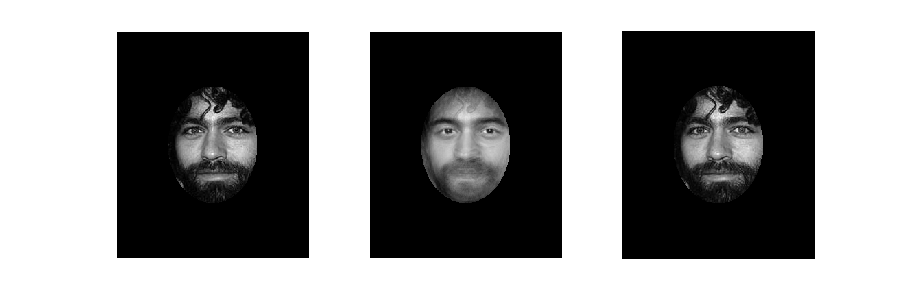
\includegraphics[width=180mm]{images/celeb1.png}
\label{overflow}
\end{figure} \\
Celebrity 2:
\begin{figure}[ht!]
\centering
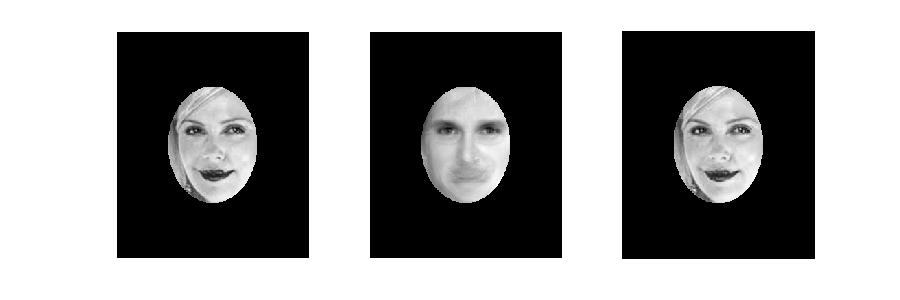
\includegraphics[width=180mm]{images/celeb2.png}
\label{overflow}
\end{figure}
\newpage

\section*{2. Eigenfaces (page 3 out of 7)}
Celebrity 3:
\begin{figure}[ht!]
\centering
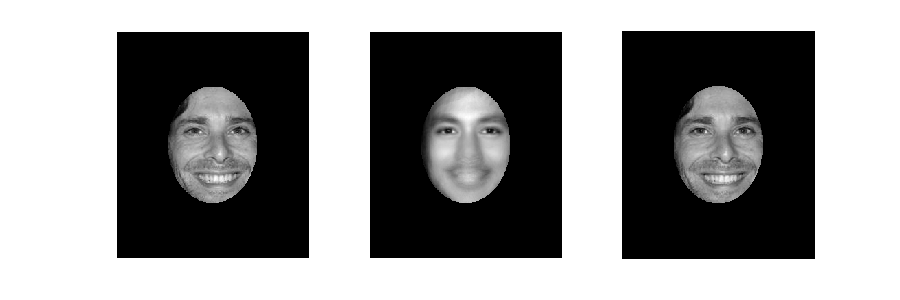
\includegraphics[width=180mm]{images/celeb3.png}
\label{overflow}
\end{figure} \\
Celebrity 4:
\begin{figure}[ht!]
\centering
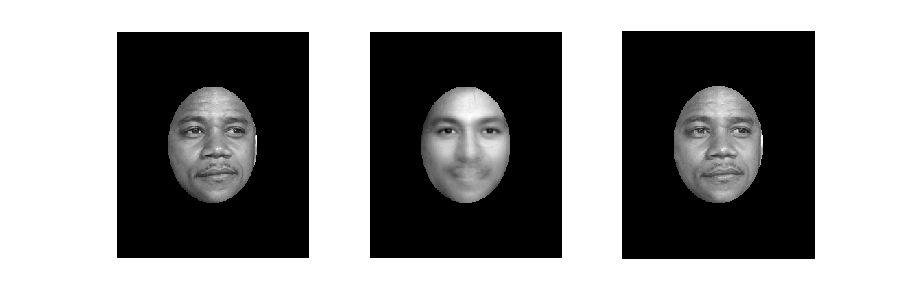
\includegraphics[width=180mm]{images/celeb4.png}
\label{overflow}
\end{figure} \\
Celebrity 5:
\begin{figure}[ht!]
\centering
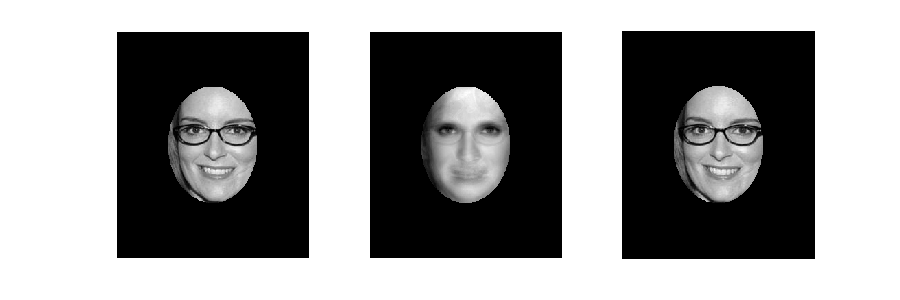
\includegraphics[width=180mm]{images/celeb5.png}
\label{overflow}
\end{figure}
\newpage

\section*{2. Eigenfaces (page 4 out of 7)}
Analysis: The reconstructions are what we expect. Even with 10 eigenvectors, we can see the structure of the person's face. For example, the reconstruction of celebrity 1, who has a lot of facial hair and hair, is also showing signs of dark areas near the mouth and forehead. Celebrity 5, who is wearing glasses, gets a faint reconstruction of glasses with 10 eigenvectors. As we ramp up the number of eigenvectors to 130, we see that the reconstruction is nearly perfect. Here is a plot for the reconstruction L2 error (distance between the reconstructed face and the actual face) versus the top $k$ eigenvectors used. Note that the  error gradually decreases as we add more eigenvectors. When using all 158 eigenvectors, the reconstruction becomes perfect (0 error). \\
\begin{figure}[ht!]
\centering
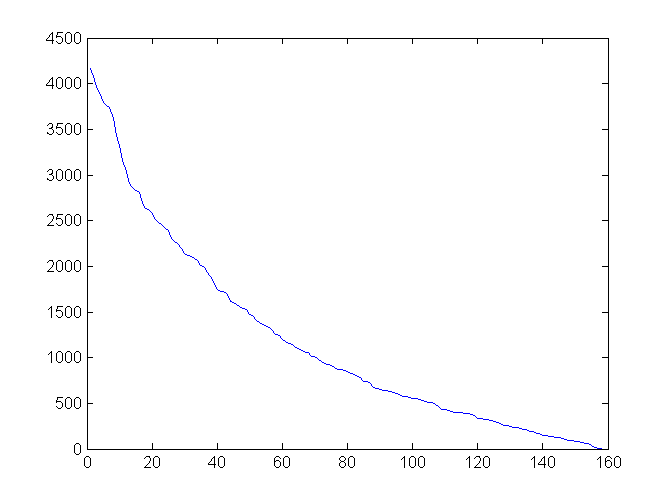
\includegraphics[width=180mm]{images/hw7q2berror.png}
\label{overflow}
\end{figure} \\
Above: x-axis: number of eigenvectors, y-axis: L2 reconstruction error. \\\\
Run hw7q2b in the code subdirectory to reproduce this graph. (though, it uses a random 5 samples)
\newpage

\section*{2. Eigenfaces (page 5 out of 7)}
(c) We randomly pick 5 student faces to reconstruct from the eigenvectors found from our celebrity database. Similarly, each student with have 3 images, the first being the actual image, the second being the reconstructed image with the top 20 celebrity eigenvectors (from the spces), and the third being the reconstructed image with all 158 celebrity eigenvectors. \\\\
Student 1:
\begin{figure}[ht!]
\centering
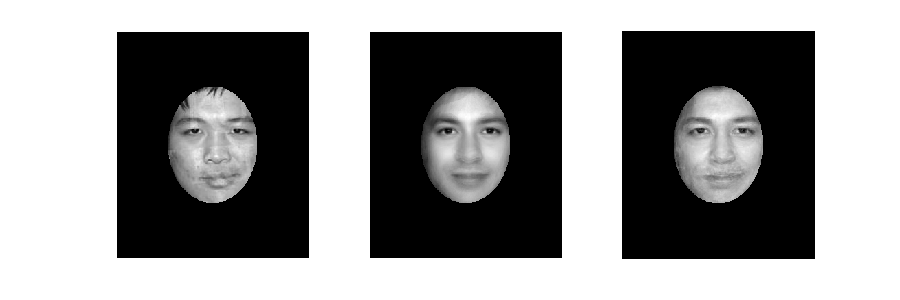
\includegraphics[width=180mm]{images/student1.png}
\label{overflow}
\end{figure} \\
Student 2:
\begin{figure}[ht!]
\centering
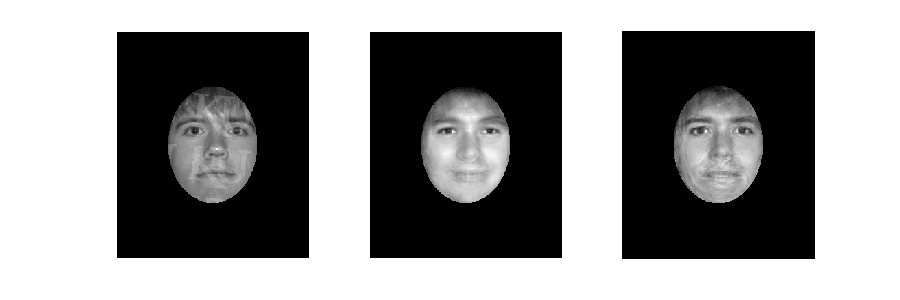
\includegraphics[width=180mm]{images/student2.png}
\label{overflow}
\end{figure}
\newpage

\section*{2. Eigenfaces (page 6 out of 7)}
Student 3:
\begin{figure}[ht!]
\centering
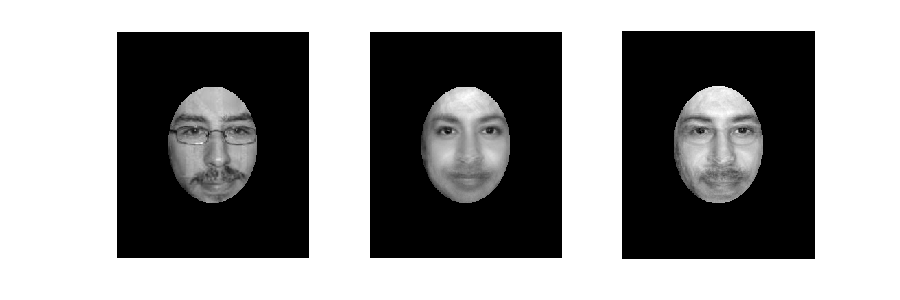
\includegraphics[width=180mm]{images/student3.png}
\label{overflow}
\end{figure} \\
Student 4:
\begin{figure}[ht!]
\centering
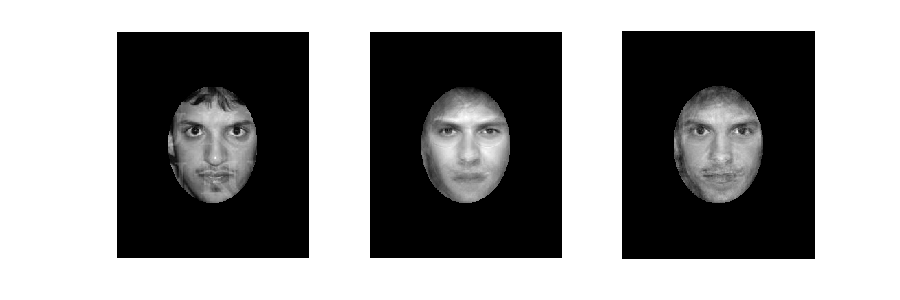
\includegraphics[width=180mm]{images/student4.png}
\label{overflow}
\end{figure} \\
Student 5:
\begin{figure}[ht!]
\centering
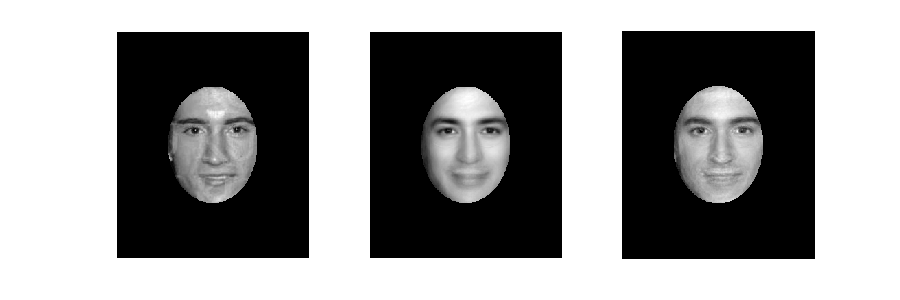
\includegraphics[width=180mm]{images/student5.png}
\label{overflow}
\end{figure}
\newpage

\section*{2. Eigenfaces (page 7 out of 7)}
Analysis: As expected, the reconstruction of images not seen by the PCA algorithm will not be perfectly reconstructed. This is because we're trying to represent a never-before seen image with only components from 158 celebrities. Though the reconstruction isn't perfect, the student reconstructions didn't turn out too poorly. With only 20 eigenvectors from the celebrity images, we can already see the structure of the students' faces. With 158 eigenvectors, the images turn out pretty nicely. For example, see student 3: his moustache and glasses show correctly. Here is a plot for the reconstruction L2 error (distance between the reconstructed face and the actual face) versus the top $k$ eigenvectors used. As stated above, the reconstruction error decreases, but it will not reach 0. \\
\begin{figure}[ht!]
\centering
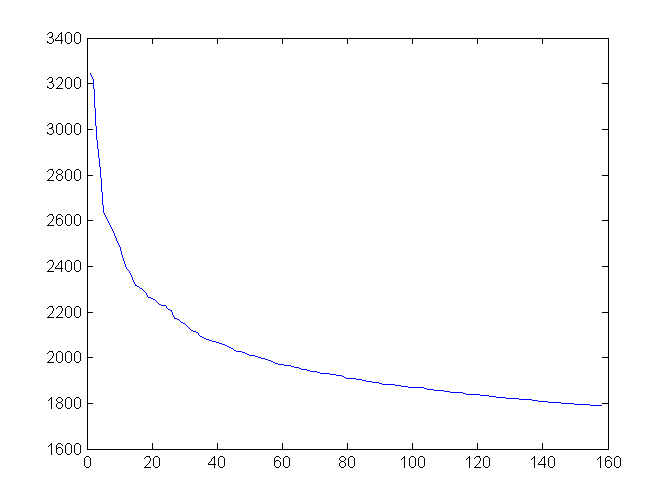
\includegraphics[width=180mm]{images/hw7q2cerror.png}
\label{overflow}
\end{figure} \\
Above: x-axis: number of eigenvectors, y-axis: L2 reconstruction error. \\\\
Run hw7q2c in the code subdirectory to reproduce this graph. (though, it uses a random 5 samples)
\newpage



\section*{3. SVD Practice (page 1 out of 4)}
a) $ A = \begin{bmatrix}
2 & 2 \\
1 & -1 \\
\end{bmatrix} $ \\\\
\textbf{(1) Compute $U$ by calculating eigenvectors of $AA^T$.}
\\\\
$AA^T = \begin{bmatrix}
2 & 2 \\
1 & -1 \\
\end{bmatrix} \begin{bmatrix}
2 & 1 \\
2 & -1 \\
\end{bmatrix} = \begin{bmatrix}
8 & 0 \\
0 & 2 \\
\end{bmatrix} $ \\\\
The eigenvalues of $AA^T$ will satisfy $det(A - \lambda I ) = 0$. First, let's compute $A - \lambda I$: \\\\
$ A - \lambda I = \begin{bmatrix}
8 & 0 \\
0 & 2 \\
\end{bmatrix} - \begin{bmatrix}
\lambda & 0 \\
0 & \lambda \\
\end{bmatrix} = \begin{bmatrix}
8 - \lambda & 0 \\
0 & 2 - \lambda \\
\end{bmatrix}$ \\\\
$det(A - \lambda I) = (8 - \lambda) (2 - \lambda)$. \\
Setting the determinant equal to 0 and solving for $\lambda$, we get: $\lambda = 2, 8.$ \\\\
Now we have to find the associated eigenvectors for each eigenvalue. Particularly, we're looking for a $v$ such that $Av = \lambda v$, or, in other words, $(A - \lambda I)v = 0$. \\\\
Let $\lambda = 8$, then $(A - \lambda I) = \begin{bmatrix}
8 - \lambda & 0 \\
0 & 2 - \lambda \\
\end{bmatrix} = \begin{bmatrix}
0 & 0 \\
0 & -6 \\
\end{bmatrix}$. \\\\
Letting $(A - \lambda I)v = 0$, we get that $ \begin{bmatrix}
0 & 0 \\
0 & -6 \\
\end{bmatrix} \begin{bmatrix}
v_0 \\
v_1 \\
\end{bmatrix} = \begin{bmatrix}
0 \\
-6v_1 \\
\end{bmatrix} = \begin{bmatrix}
0 \\
0 \\
\end{bmatrix} $. \\\\
For this equality to hold, $v_1$ must be 0. We want the vector to be orthonormal, so set $v_0 =1$. \\\\
Then: $v = \begin{bmatrix}
1 \\
0 \\
\end{bmatrix}$ is an eigenvector for eigenvalue $\lambda = 8$. \\\\
Let $\lambda = 2$, then $(A - \lambda I) = \begin{bmatrix}
8 - \lambda & 0 \\
0 & 2 - \lambda \\
\end{bmatrix} = \begin{bmatrix}
6 & 0 \\
0 & 0 \\
\end{bmatrix}$. \\\\
Letting $(A - \lambda I)v = 0$, we get that $ \begin{bmatrix}
6 & 0 \\
0 & 0 \\
\end{bmatrix} \begin{bmatrix}
v_0 \\
v_1 \\
\end{bmatrix} = \begin{bmatrix}
6v_0 \\
0 \\
\end{bmatrix} = \begin{bmatrix}
0 \\
0 \\
\end{bmatrix} $. \\\\
For this equality to hold, $v_0$ must be 0. We want the vector to be orthonormal, so set $v_1 = 1$. \\\\
Then: $v = \begin{bmatrix}
0 \\
1 \\
\end{bmatrix}$ is an eigenvector for eigenvalue $\lambda = 2$. \\\\
We'll define $U$ as a 2x2 matrix, where each column contains the corresponding eigenvalues we found:
Hence:
$$ \boxed{ U = \begin{bmatrix} 
v_{\lambda = 8} & v_{\lambda = 2} \\
\end{bmatrix} = \begin{bmatrix}
1 & 0\\
0 & 1\\
\end{bmatrix}}$$
\textbf{(2) Compute the entries of $\Sigma$ by calculating the positive square roots of the eigenvalues of $AA^T$.}
\\\\
Since we found the eigenvalues in part (1), we just take the square roots of them and place them in the diagonal matrix corresponding to the order of the eigenvectors in $U$.
$$\boxed{\Sigma = diag(\sqrt8, \sqrt2) = \begin{bmatrix}
2\sqrt2 & 0 \\
0 & \sqrt2 \\
\end{bmatrix}} $$

\newpage

\section*{3. SVD Practice (page 2 out of 4)}
\textbf{(3) Compute $V$ by calculating eigenvectors of $A^TA$.}
\\\\
$A^T A= \begin{bmatrix}
2 & 1 \\
2 & -1 \\
\end{bmatrix} \begin{bmatrix}
2 & 2 \\
1 & -1 \\
\end{bmatrix} = \begin{bmatrix}
5 & 3 \\
3 & 5 \\
\end{bmatrix} $ \\\\
The eigenvalues of $AA^T$ will satisfy $det(A - \lambda I ) = 0$. First, let's compute $A - \lambda I$: \\\\
$ A - \lambda I = \begin{bmatrix}
5 & 3 \\
3 & 5 \\
\end{bmatrix} - \begin{bmatrix}
\lambda & 0 \\
0 & \lambda \\
\end{bmatrix} = \begin{bmatrix}
5 - \lambda & 3 \\
3 & 5 - \lambda \\
\end{bmatrix}$ \\\\
$det(A - \lambda I) = (5 - \lambda)^2 - 9 = \lambda^2 - 10\lambda + 16 = (\lambda - 8)(\lambda - 2)$. \\
Setting the determinant equal to 0 and solving for $\lambda$, we get: $\lambda = 2, 8.$ \\\\
Now we have to find the associated eigenvectors for each eigenvalue. Particularly, we're looking for a $v$ such that $Av = \lambda v$, or, in other words, $(A - \lambda I)v = 0$. \\\\
Let $\lambda = 8$, then $(A - \lambda I) = \begin{bmatrix}
5 - \lambda & 3 \\
3 & 5 - \lambda \\
\end{bmatrix} = \begin{bmatrix}
-3 & 3 \\
3 & -3 \\
\end{bmatrix}$. \\\\
Letting $(A - \lambda I)v = 0$, we get that $ \begin{bmatrix}
-3 & 3 \\
3 & -3 \\
\end{bmatrix} \begin{bmatrix}
v_0 \\
v_1 \\
\end{bmatrix} = \begin{bmatrix}
-3v_0 + 3v_1 \\
3v_0 -3v_1 \\
\end{bmatrix} = \begin{bmatrix}
0 \\
0 \\
\end{bmatrix} $. \\\\
For this equality to hold, $v_0 = v_1$. We want the vector to be orthonormal, so set $v_0 = 1 / \sqrt2$ and $v_1 = 1 / \sqrt2.$ \\\\
Then: $v = \begin{bmatrix}
1 / \sqrt2 \\
1 / \sqrt2 \\
\end{bmatrix}$ is an eigenvector for eigenvalue $\lambda = 8$. \\\\
Let $\lambda = 2$, then $(A - \lambda I) = \begin{bmatrix}
5 - \lambda & 3 \\
3 & 5 - \lambda \\
\end{bmatrix} = \begin{bmatrix}
3 & 3 \\
3 & 3 \\
\end{bmatrix}$. \\\\
Letting $(A - \lambda I)v = 0$, we get that $ \begin{bmatrix}
3 & 3 \\
3 & 3 \\
\end{bmatrix} \begin{bmatrix}
v_0 \\
v_1 \\
\end{bmatrix} = \begin{bmatrix}
3v_0 + 3v_1 \\
3v_0 + 3v_1 \\
\end{bmatrix} = \begin{bmatrix}
0 \\
0 \\
\end{bmatrix} $. \\\\
For this equality to hold, $v_0 = -v_1$. We want the vector to be orthonormal, so set $v_0 = 1 / \sqrt2$ and $v_1 = - 1 / \sqrt2.$ \\\\
Then: $v = \begin{bmatrix}
1 / \sqrt2 \\
- 1 / \sqrt2 \\
\end{bmatrix}$ is an eigenvector for eigenvalue $\lambda = 2$. \\\\
We'll define $V$ as a 2x2 matrix, where each column contains the corresponding eigenvalues we found:
Hence:
$$ \boxed{ V = \begin{bmatrix} 
v_{\lambda = 8} & v_{\lambda = 2} \\
\end{bmatrix} = \begin{bmatrix}
1 / \sqrt2 & 1 / \sqrt2 \\
1 / \sqrt2 & -1 / \sqrt2 \\
\end{bmatrix}}$$
\textbf{(4) Verify that $A = U \Sigma V^T.$}
$$\begin{aligned}
U \Sigma V^T &= \begin{bmatrix}
1 & 0 \\
0 & 1 \\
\end{bmatrix} \begin{bmatrix}
2 \sqrt2 & 0 \\
0 & \sqrt2 \\
\end{bmatrix} \begin{bmatrix}
1 / \sqrt2 & 1 / \sqrt2 \\
1 / \sqrt2 & -1 / \sqrt2 \\
\end{bmatrix} \\
&= \begin{bmatrix}
2 \sqrt2 & 0 \\
0 & \sqrt2 \\
\end{bmatrix} \begin{bmatrix}
1 / \sqrt2 & 1 / \sqrt2 \\
1 / \sqrt2 & -1 / \sqrt2 \\
\end{bmatrix} \\
&= \begin{bmatrix}
2 & 2 \\
1 & -1 \\
\end{bmatrix} \\
&= \boxed{A}
\end{aligned} $$


\section*{3. SVD Practice (page 3 out of 4)}
a) $ A = \begin{bmatrix}
2 & 2 \\
1 & 1 \\
\end{bmatrix} $ \\\\
\textbf{(1) Compute $U$ by calculating eigenvectors of $AA^T$.}
\\\\
$AA^T = \begin{bmatrix}
2 & 2 \\
1 & 1 \\
\end{bmatrix} \begin{bmatrix}
2 & 1 \\
2 & 1 \\
\end{bmatrix} = \begin{bmatrix}
8 & 4 \\
4 & 2 \\
\end{bmatrix} $ \\\\
The eigenvalues of $AA^T$ will satisfy $det(A - \lambda I ) = 0$. First, let's compute $A - \lambda I$: \\\\
$ A - \lambda I = \begin{bmatrix}
8 & 4 \\
4 & 2 \\
\end{bmatrix} - \begin{bmatrix}
\lambda & 0 \\
0 & \lambda \\
\end{bmatrix} = \begin{bmatrix}
8 - \lambda & 4 \\
4 & 2 - \lambda \\
\end{bmatrix}$ \\\\
$det(A - \lambda I) = (8 - \lambda) (2 - \lambda) - 16 = \lambda^2 - 10\lambda + 16 - 16 = \lambda (\lambda - 10)$. \\
Setting the determinant equal to 0 and solving for $\lambda$, we get: $\lambda = 0, 10.$ \\\\
Now we have to find the associated eigenvectors for each eigenvalue. Particularly, we're looking for a $v$ such that $Av = \lambda v$, or, in other words, $(A - \lambda I)v = 0$. \\\\
Let $\lambda = 10$, then $(A - \lambda I) = \begin{bmatrix}
8 - \lambda & 4 \\
4 & 2 - \lambda \\
\end{bmatrix} = \begin{bmatrix}
-2 & 4 \\
4 & -8 \\
\end{bmatrix}$. \\\\
Letting $(A - \lambda I)v = 0$, we get that $ \begin{bmatrix}
-2 & 4 \\
4 & -8 \\
\end{bmatrix} \begin{bmatrix}
v_0 \\
v_1 \\
\end{bmatrix} = \begin{bmatrix}
-2v_0 + 4v_1 \\
4v_0 - 8v_1 \\
\end{bmatrix} = \begin{bmatrix}
0 \\
0 \\
\end{bmatrix} $. \\\\
For this equality to hold, $v_0 = 2v_1$. We want the vector to be orthonormal, so set $v_0 = 2 / \sqrt5$ and $v_1 = 1 / \sqrt5.$ \\\\
Then: $v = \begin{bmatrix}
2 / \sqrt5 \\
1 / \sqrt5 \\
\end{bmatrix}$ is an eigenvector for eigenvalue $\lambda = 10$. \\\\
Let $\lambda = 0$, then $(A - \lambda I) = \begin{bmatrix}
8 - \lambda & 4 \\
4 & 2 - \lambda \\
\end{bmatrix} = \begin{bmatrix}
8 & 4 \\
4 & 2 \\
\end{bmatrix}$. \\\\
Letting $(A - \lambda I)v = 0$, we get that $ \begin{bmatrix}
8 & 4 \\
4 & 2 \\
\end{bmatrix} \begin{bmatrix}
v_0 \\
v_1 \\
\end{bmatrix} = \begin{bmatrix}
8v_0 + 4v_1 \\
4v_0 + 2v_1 \\
\end{bmatrix} = \begin{bmatrix}
0 \\
0 \\
\end{bmatrix} $. \\\\
For this equality to hold, $-2v_0 = v_1$. We want the vector to be orthonormal, so set $v_0 = 1 / \sqrt5$ and $v_1 = - 2 / \sqrt5.$ \\\\
Then: $v = \begin{bmatrix}
1 / \sqrt5 \\
-2 / \sqrt5 \\
\end{bmatrix}$ is an eigenvector for eigenvalue $\lambda = 0$. \\\\
We'll define $U$ as a 2x2 matrix, where each column contains the corresponding eigenvalues we found:
Hence:
$$ \boxed{ U = \begin{bmatrix} 
v_{\lambda = 10} & v_{\lambda = 0} \\
\end{bmatrix} = \begin{bmatrix}
2 / \sqrt5 & 1 / \sqrt5 \\
1 / \sqrt5 & -2 / \sqrt5 \\
\end{bmatrix}}$$
\textbf{(2) Compute the entries of $\Sigma$ by calculating the positive square roots of the eigenvalues of $AA^T$.}
\\\\
Since we found the eigenvalues in part (1), we just take the square roots of them and place them in the diagonal matrix corresponding to the order of the eigenvectors in $U$.
$$\boxed{\Sigma = diag(\sqrt{10}, 0) = \begin{bmatrix}
\sqrt{10} & 0 \\
0 & 0 \\
\end{bmatrix}} $$

\newpage

\section*{3. SVD Practice (page 4 out of 4)}
\textbf{(3) Compute $V$ by calculating eigenvectors of $A^TA$.}
\\\\
$A^T A= \begin{bmatrix}
2 & 1 \\
2 & 1 \\
\end{bmatrix} \begin{bmatrix}
2 & 2 \\
1 & 1 \\
\end{bmatrix} = \begin{bmatrix}
5 & 5 \\
5 & 5 \\
\end{bmatrix} $ \\\\
The eigenvalues of $AA^T$ will satisfy $det(A - \lambda I ) = 0$. First, let's compute $A - \lambda I$: \\\\
$ A - \lambda I = \begin{bmatrix}
5 & 5 \\
5 & 5 \\
\end{bmatrix} - \begin{bmatrix}
\lambda & 0 \\
0 & \lambda \\
\end{bmatrix} = \begin{bmatrix}
5 - \lambda & 5 \\
5 & 5 - \lambda \\
\end{bmatrix}$ \\\\
$det(A - \lambda I) = (5 - \lambda)^2 - 25 = \lambda^2 - 10\lambda + 25 - 25 = \lambda(\lambda - 10)$. \\
Setting the determinant equal to 0 and solving for $\lambda$, we get: $\lambda = 0, 10.$ \\\\
Now we have to find the associated eigenvectors for each eigenvalue. Particularly, we're looking for a $v$ such that $Av = \lambda v$, or, in other words, $(A - \lambda I)v = 0$. \\\\
Let $\lambda = 10$, then $(A - \lambda I) = \begin{bmatrix}
5 - \lambda & 5 \\
5 & 5 - \lambda \\
\end{bmatrix} = \begin{bmatrix}
-5 & 5 \\
5 & -5 \\
\end{bmatrix}$. \\\\
Letting $(A - \lambda I)v = 0$, we get that $ \begin{bmatrix}
-5 & 5 \\
5 & -5 \\
\end{bmatrix} \begin{bmatrix}
v_0 \\
v_1 \\
\end{bmatrix} = \begin{bmatrix}
-5v_0 + 5v_1 \\
5v_0 -5v_1 \\
\end{bmatrix} = \begin{bmatrix}
0 \\
0 \\
\end{bmatrix} $. \\\\
For this inequality to hold, $v_0 = v_1$. We want the vector to be orthonormal, so set $v_0 = 1 / \sqrt2$ and $v_1 = 1 / \sqrt2.$ \\\\
Then: $v = \begin{bmatrix}
1 / \sqrt2 \\
1 / \sqrt2 \\
\end{bmatrix}$ is an eigenvector for eigenvalue $\lambda = 10$. \\\\
Let $\lambda = 0$, then $(A - \lambda I) = \begin{bmatrix}
5 - \lambda & 5 \\
5 & 5 - \lambda \\
\end{bmatrix} = \begin{bmatrix}
5 & 5 \\
5 & 5 \\
\end{bmatrix}$. \\\\
Letting $(A - \lambda I)v = 0$, we get that $ \begin{bmatrix}
5 & 5 \\
5 & 5 \\
\end{bmatrix} \begin{bmatrix}
v_0 \\
v_1 \\
\end{bmatrix} = \begin{bmatrix}
5v_0 + 5v_1 \\
5v_0 + 5v_1 \\
\end{bmatrix} = \begin{bmatrix}
0 \\
0 \\
\end{bmatrix} $. \\\\
For this inequality to hold, $v_0 = -v_1$. We want the vector to be orthonormal, so set $v_0 = 1 / \sqrt2$ and $v_1 = - 1 / \sqrt2.$ \\\\
Then: $v = \begin{bmatrix}
1 / \sqrt2 \\
- 1 / \sqrt2 \\
\end{bmatrix}$ is an eigenvector for eigenvalue $\lambda = 0$. \\\\
We'll define $V$ as a 2x2 matrix, where each column contains the corresponding eigenvalues we found:
Hence:
$$ \boxed{ V = \begin{bmatrix} 
v_{\lambda = 10} & v_{\lambda = 0} \\
\end{bmatrix} = \begin{bmatrix}
1 / \sqrt2 & 1 / \sqrt2 \\
1 / \sqrt2 & -1 / \sqrt2 \\
\end{bmatrix}}$$
\textbf{(4) Verify that $A = U \Sigma V^T.$}
$$\begin{aligned}
U \Sigma V^T &=\begin{bmatrix}
2 / \sqrt5 & 1 / \sqrt5 \\
1 / \sqrt5 & -2 / \sqrt5 \\
\end{bmatrix} \begin{bmatrix}
\sqrt{10} & 0 \\
0 & 0 \\
\end{bmatrix} \begin{bmatrix}
1 / \sqrt2 & 1 / \sqrt2 \\
1 / \sqrt2 & -1 / \sqrt2 \\
\end{bmatrix} \\
&= \begin{bmatrix}
2 \sqrt2 & 0\\
\sqrt2 & 0 \\
\end{bmatrix} \begin{bmatrix}
1 / \sqrt2 & 1 / \sqrt2 \\
1 / \sqrt2 & -1 / \sqrt2 \\
\end{bmatrix} \\
&= \begin{bmatrix}
2 & 2 \\
1 & 1 \\
\end{bmatrix} \\
&= \boxed{A}
\end{aligned} $$

\end{document}